\section{Design}
\label{Design}

\begin{figure}[ht]
\begin{centering}
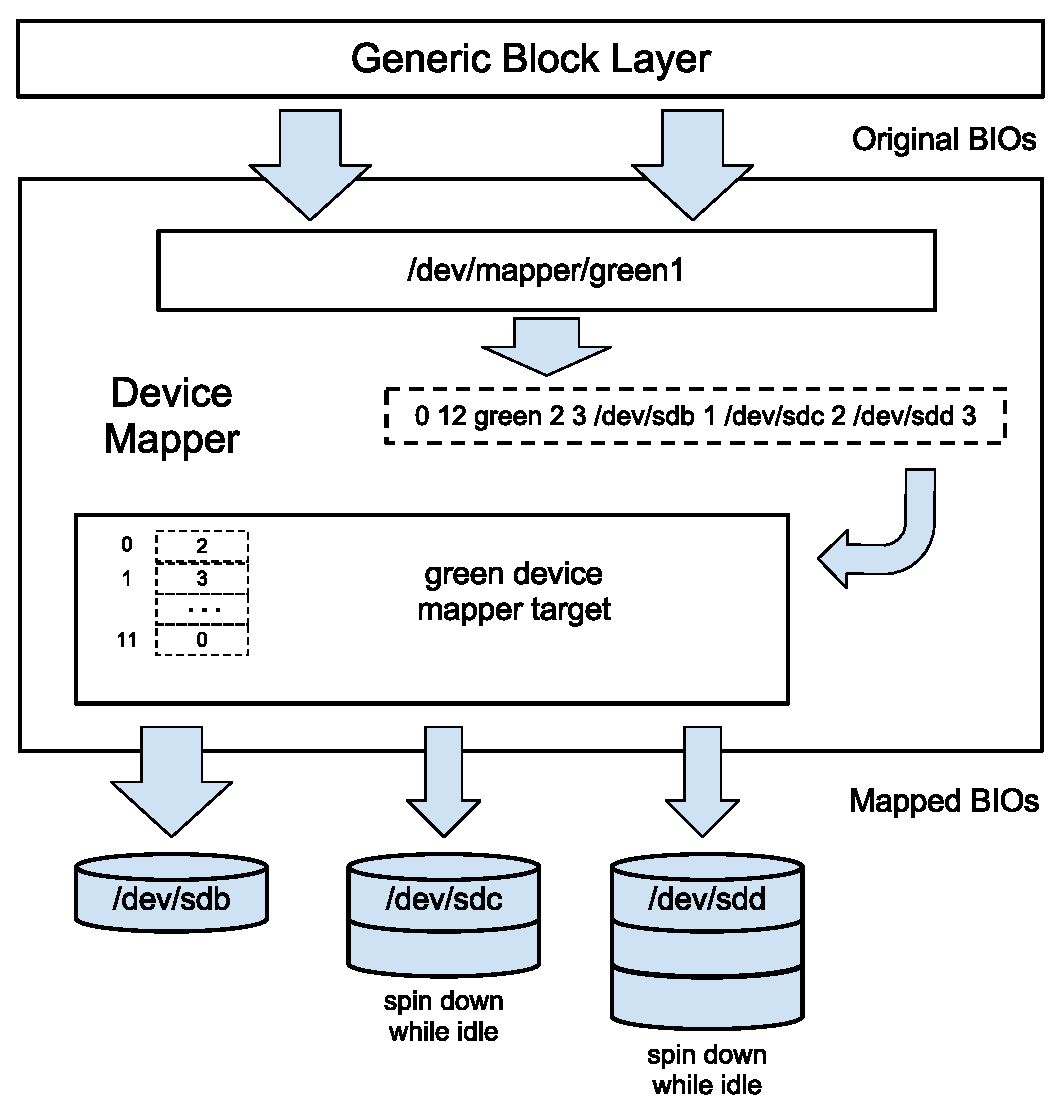
\epsfig{file=figures/dm.eps,width=1.00\linewidth}
\caption{Linux Device Mapper and Green Device Mapper Target.
/dev/mapper/green1 is a virtual block device. The two dashed boxes are
mapping tables. The first one is used by Device Mapper to delegate
mapping to target; the second one is used internally by the green
target.}
\label{fig:dm}
\end{centering}
\end{figure}

We present the design of our green multi-disk driver as a Linux Device
Mapper target. Linux Device Mapper, as depicted in Figure
\ref{fig:dm}, is a generic framework to map one block device onto
another. It works by processing data passed in from a virtual block
device, that it itself provides, and then passing the resultant data
on to another block device. The advantage of Device Mapper is that it
can provide virtual devices to user programs and kernel modules above
block level without exposing details of underlying devices. Thanks to
this transparency, the underlying devices can be of different size and
type (can in turn be virtual or physical) and the mapping can be
performed in different ways. Device mapper is essentially a
middle-ware sitting between the Generic Block Layer and block devices.
It receives BIOs, which is a kernel structure describe I/O requests,
from Generic Block Layer, then redirect them to other block devices by
modifying the target device and target sector. 

Device Mapper itself does not perform the redirection. It delegates
this operation to Device Mapper targets, which are registered kernel
modules performing certain kinds of mapping. This delegation is
specified in a mapping table, which contains the type of responsible
Device Mapper target for certain regions of block devices. In Figure
\ref{fig:dm}, all I/O request to sectors [0, 0+12) of virtual device
"/dev/mapping/green1" will be handled by a target named green; all
parameters after "green" are passed to the green target. A mapping
target which contains functions to construct/destruct mapped devices,
map I/O requests, merge adjacent I/O requests, report and control
device status.

\subsection{Design Goals}
The design goal of our green multi-disk driver is driven by the
following guiding principles: 

\begin{itemize}
\item \textbf{Save energy by allowing disks to spin/power down}. Be
energy efficiency is one of the most important feature our green
multi-disk driver is pursuing. The SSD cache benefits both I/O
performance and energy efficiency benefit. In this study, we are more
concerned of the latter and there is tradeoff between the two. 

\item \textbf{Use SSD aware data structures and algorithms}. While SSD
provides better I/O performance and energy efficency, it has its own
constraints including limited eraze-write cycles and inefficient
random writes. This principle guides our design to avoid these
constraints and extract maximum benefit out of SSD.

\item \textbf{Provide stable and robust storage}. Because our green
target provides customized data mapping and block grouping, it is
critical to always perform correct translation between virtual and
physical blocks. It should not lose data in case of power failure or
other hazardous conditions.
\end{itemize}

\subsection{Disk Management}

Device Mapper targets maintain mapping of sectors between virtual and
physical disks. The straightforward method is to maintain a
sector-wise mapping table. However, it is prohibitive because its size
is too large to fit in memory. For example, the size of sector-wise
mapping table of a 1TB disk (512-byte sectors) is as large as 8GB with
4-bytes table entries. Store the mapping table on disk (even on SSD)
is not an option because it is too slow to incur extra I/O. A solution
is to divide disks into larger unit. Here, we adopt the LVM term
extent, which is the unit of disk managed by LVM, typically 4MB. Then
the mapping becomes extent-wise and its size diminishes to 1MB in the
above example. 

In the green target, multiple physical disks are mapped as a single
virtual disk. They will be kept in the order of energy efficiency,
i.e., the most energy-efficient goes first and so on. In Figure
\ref{fig:dm}, '/dev/sdb' is the most energy-efficient one but with
smallest capacity, i.e., SSD; '/dev/sdc' and '/dev/sdd' follow
decreasingly in energy-efficiency and increasingly in capacity. This
makes the addressing of physical sectors easy. An extent index and an
offset within extent suffice. We have noticed the case that one IO
request on logically sequential blocks might be mapped to multiple IO
requests on physically non-sequential blocks. Therefore, the
translation is performed per extent instead of per request. However,
extent is of big size, so it is unlikely that the extent by extent
translation is a performance bottleneck. It is not a problem also
because the Device Mapper framework provides interface to merge
adjacent I/O requests. 

The exact size of extent is an important factor as it affects not only
memory consumption but also granularity of mapping. A large size of
extent has the following impacts: 

\begin{itemize} 
\item \textbf{Smaller mapping table}. As already discussed, the
adoption of extent makes the mapping table becomes extent-wise and its
size is reduced. 

\item \textbf{More aggresive prefetch}. As energy-efficient disk such
as SSD have similar effect as disk cache. When a large extent of data
is move onto SSD, it can be consider as an aggresive prefetch. 

\item \textbf{Coarse-grain data migration among disks and more
sequential I/O}. Because the major lantency of magnetic disk is seek
time, a larger sequential access will not significantly slow down the
IO. Moreover, with large size of migration unit, there are fewer IO
because adjacent sectors can be grouped. This is benefical to the life
time of SSD as well considering its limited write-erase cycles.

\item \textbf{High overhead}. Since each extent can represent several
sectors, depends on the workload IO, more sectors IO can be wasteful
and only adds overhead to the overall system. 

\end{itemize}

Different workloads might also favor different extent sizes
considering file sizes and I/O frequency. Therefore, we make it a
configurable parameter to the green target so that different
trade-offs can be made by configuration. 

\subsection{Mapping Table}

There are two mapping tables. One is actually a configuration file
used by the Device Mapper framework; the other contains extent-wise
mapping information used internally by our green target. We are
talking about the second one in following discussion. 

The straightforward structure of the mapping table is an array of the
size of total extent number. The mapping table is maintained in memory
and can be cached, so its lookup is fast. Besides mapping information,
the table also contains other fields including flags, timestamp of the
latest access and number of total access (possibly distinguished
between read and write). Flags are used to record states of extents,
which may include for example 1) whether the extent is accessed or
not; 2) whether the extent is under migration or not; and 3) whether
the extent is updated or not when it is under migration. Timestamp of
the latest access and number of total access are used to predict hot
extent. Their use will be discussed in next section. 

The mapping table need be saved to disk on power off as metadata. To
be fail-safe, it has a replicate in every physical disk. The in-memory
version and on-disk version of mapping table can be slightly
different, since it is not necessary to save online information such
as timestamp of latest access. Moreover, to be robust in case of
hazardous situation such as power failure, the mapping table is
flushed onto disk periodically. To prevent this periodical background
job from interrupting other disk, it only save the table on the cache
disk. Table on other disks are only updated on request or when the
system is being shutting down.

%-----------------------------------------------------------------------------

\subsection{Extent Migration}
There are two kind of extent movements. The first is the movement
between the SSD cache disk and secondary disks. The second is the
movement between secondary disks. The first kind of movement is
actually cache loading and eviction. It is neccessary for ensuring
that we always maintain hot extents on cache disk. LRU algorithm is
used in this case. The second movement, which is extent migration,
happens when there is a need to keep all extents of a working set on a
single physical disk. 

\subsection{Trace Study}

Trace analysis plays a crucial role in identifying hot data blocks
across different disks. The idea is to move hot blocks to cache disk
and serve most of the requests from the energy-efficient cache disk
and hence spin/power down other secondary disks for long periods of
time to achieve good power savings and increased performance. I/O
block traces can be used both in offline mode and online mode. In
offline mode, first we collect traces for a particular workload and
later analyze these traces to tweak important parameters. For example,
a good value for parameters like extent size and migration threshold
can be decided by studying the traces for a workload. In online mode,
we use I/O block traces to dynamically identify hot blocks across
different disks. First, the traces are collected for a particular
workload and analyze these traces to identify any patterns in the I/O
accesses. If we can find a particular trend in workloads (which is
more likely for server workloads), we use trace analysis to
dynamically identify hot working sets. Workloads for video servers and
file servers are more likely to exhibit good data locality property as
only a fraction of files are popular at a particular instant and the
distribution of popular files on disks change dynamically. Also We
expect IOs of these workloads to be largely sequential in nature.
Sequential workloads are more suitable for this approach 

Right now, we use I/O traces for analysis and tweaking parameters. I/O
traces can also be used in online mode to predict the hot blocks. This
approach is another option and we may implement this if time permits.
Also, to verify the correctness and working of our concept, We will
replay the traces with and without green Multi-disk target and compare
the power consumption and I/O performance. 

We ran the workloads for a relatively long periods (for a few hours).
We used blktrace tool to collect traces. Block traces would contain
information like disk major and minor number, disk offset, number of
blocks accessed , Read/Write information  and timestamp for every I/O
sent to disk. We us the pertinent I/O information from the traces to
identify workload characteristics.

\begin{figure}[ht]
\begin{centering}
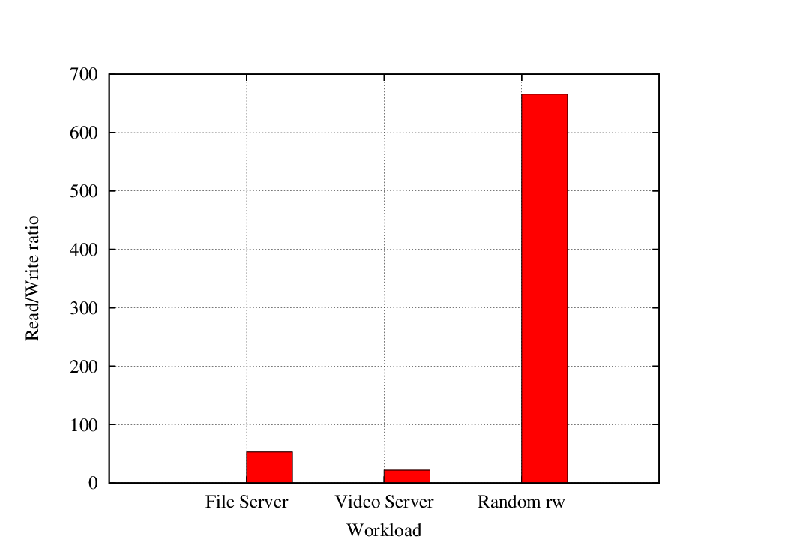
\epsfig{file=figures/rw.eps,width=1.00\linewidth}
\caption{Read/Write Ratio from Analysis of Workload Traces.}
\label{fig:rw}
\end{centering}
\end{figure}

In Figure \ref{fig:rw}, we present the graphs for Read/Write ratio for
three different workloads, namely random read/write, videoserver and
fileserver workloads. All these workloads were generated using
filebench and each workload was run for 2 hours. We used three
different physical disks with different power consumption and
performance characteristics to run these workloads.   

%%%%%%%%%%%%%%%%%%%%%%%%%%%%%%%%%%%%%%%%%%%%%%%%%%%%%%%%%%%%%%%%%%%%%%%%%%%%%%
%% For Emacs:
% Local variables:
% fill-column: 70
% End:
%%%%%%%%%%%%%%%%%%%%%%%%%%%%%%%%%%%%%%%%%%%%%%%%%%%%%%%%%%%%%%%%%%%%%%%%%%%%%%
%% For Vim:
% vim:textwidth=70
%%%%%%%%%%%%%%%%%%%%%%%%%%%%%%%%%%%%%%%%%%%%%%%%%%%%%%%%%%%%%%%%%%%%%%%%%%%%%%
% LocalWords:  
